\chapter{多尺度食品热状态：从多孔介质到决策流形}
\label{ch:physics}

本章要判定的量是：停机、探针和解释至少要看见哪几个场，以及哪一组泛函足够支撑这些决定。判定失败的表现是把“中心温度到了”写成品质，或把十六条控制体的工程通量写成多孔介质方程的解。

\section{计算域与状态}

\paragraph{要判定的量}
食品区域与腔体区域的边界上，哪些量属于食品状态，哪些量只作为边界输入。

\paragraph{继承的文献层与不继承的层}
体积分数的三相分解继承多孔介质平均 \cite{whitaker1977}。食品加工中的用法继承 \cite{datta2007}。不继承在孔隙尺度上跟踪每一个弯月面。不继承把腔体气体的速度场并进食品未知量。

食品区域 \(\Omega_f\subset\R^3\)，腔体气体区域 \(\Omega_c\)，交界面 \(\Gamma=\partial\Omega_f\)。时间 \(t\in[0,t_f]\)。体积分数满足
\begin{equation}
\varepsilon_s+\varepsilon_l+\varepsilon_g=1,\qquad \varepsilon_s=\varepsilon_s(S)>0.
\end{equation}
\(S(\vect{r},t)\) 综合收缩、孔隙闭合与表面结壳。它不是某一个分子机理的别名。

\begin{definition}[全场状态]
\label{def:fullstate}
\begin{equation}
\label{eq:state}
\vect{X}(\vect{r},t)=\big(T,\,p_g,\,\varepsilon_l,\,\omega_v,\,\vect{\alpha},\,S\big).
\end{equation}
\(T\) 为温度，\(p_g\) 为气相压力，\(\varepsilon_l\) 为液态水体积分数，\(\omega_v\) 为气相中水蒸气质量分数。反应进度
\begin{equation}
\vect{\alpha}=(\alpha_p,\alpha_g,\alpha_b,\alpha_m)\in[0,1]^4
\end{equation}
依次是蛋白质变性、淀粉糊化、美拉德褐变与微生物致死当量的归一化进度。
\end{definition}

腔体状态不进入食品场，而作为边界输入 \((T_\infty,Y_\infty,\vect{v}_\infty,\dot m_{\mathrm{st}},P_{\mathrm{heat}})\)。这个划分决定了在线模块可以读取的量：边界输入是执行器，不是食品的隐藏状态。

\paragraph{本节不能推出的结论}
写出全场，不能推出本次积分器推进了 \(p_g\) 和 \(\omega_v\)。那两个分量在十六条控制体里没有独立未知量。

\subsection{从代表体元到决策量}

代表体元上的平均把孔隙里的弯月面收成体积分数。决策不读取这个平均场的每一点，只读取九个泛函：冷点温度、表面平均温度、温度标准差、平均液相、表面液相、致死当量、表面褐变、结壳和失重。记这个向量为 \(\vect{z}\)。停机看的是 \(\vect{z}\) 里的冷点和致死当量，不看全场的 \(L^2\) 范数。

这条收缩有一个不能省略的条件：冷点的位置如果随脂肪夹层移动，取几何中心的温度就不是冷点。一维核把冷点定义成十六个控制体的最低温度，所以夹层可以把最低温度从对称面挪开。二维脂肪几何没有运行，不能把这个定义写成已经覆盖烤箱里的冷点云。

\section{宏观：热与三相质量}

\paragraph{要判定的量}
能量方程里必须保留的项，以及相变能不能写成无限快的代数约束。

\paragraph{继承的文献层与不继承的层}
继承体积平均后的能量、液相和蒸汽方程的结构 \cite{whitaker1977,datta2007}。不继承局部热非平衡：固、液、气在一个代表体元内用同一个 \(T\)。这个简化在蒸烤的分钟尺度上可接受，在秒级冷凝膜上只是近似。不继承某一干燥器的对流通量闭合。

忽略热局部非平衡时，
\begin{equation}
\label{eq:energy}
(\rho c)_{\mathrm{eff}}\frac{\partial T}{\partial t}
=\nabla\!\cdot\!\big(k_{\mathrm{eff}}\nabla T\big)
-\sum_{i\in\{l,v,a\}}\nabla\!\cdot\!(h_i\vect{n}_i)
-\dot m_{\mathrm{phase}}\,\Delta h_{\mathrm{vap}}
+q_{\mathrm{reac}}.
\end{equation}
右端四项依次是导热、流体携带的显热、相变潜热和反应热。有效容积热容与导热随 \(\varepsilon_l\) 和 \(S\) 变化，因此同一块食品在表面变干后导热下降。这是外干内生的机制，不是边界条件的附加说明。

液相与蒸汽：
\begin{align}
\label{eq:liquid}
\frac{\partial(\varepsilon_l\rho_l)}{\partial t}
&=-\nabla\!\cdot\!\vect{n}_l-\dot m_{\mathrm{phase}},\\
\label{eq:vapor}
\frac{\partial(\varepsilon_g\rho_g\omega_v)}{\partial t}
&=-\nabla\!\cdot\!\vect{n}_v+\dot m_{\mathrm{phase}}.
\end{align}
通量由 Darcy 渗流与 Fick 扩散合成：
\begin{align}
\vect{n}_l&=-\rho_l\frac{k_{rl}K}{\mu_l}\nabla p_l,\\
\vect{n}_v&=-\rho_g\omega_v\frac{k_{rg}K}{\mu_g}\nabla p_g
-\rho_g D_{\mathrm{eff}}\nabla\omega_v.
\end{align}
相变保持有限速率。无限快约束会把任何温度残差直接折成水分残差，使探针无法分开热阻和含水。
\begin{equation}
\label{eq:phase}
\dot m_{\mathrm{phase}}
=K_{\mathrm{ev}}\,a_w(\varepsilon_l,T)\,
\big(p_{\mathrm{sat}}(T)-p_v\big)_+
-K_{\mathrm{cd}}\,(p_v-p_{\mathrm{sat}}(T))_+.
\end{equation}
蒸制时腔体蒸汽压高，冷凝项在表面释放潜热。烤制时蒸汽压低，蒸发项吸热并留下干壳。符号由 \(p_v-p_{\mathrm{sat}}\) 决定，不由“当前模式叫做蒸还是烤”决定。

干空气通量与 \eqref{eq:vapor} 对称，相变源项改号。气相总压由状态方程闭合。这些闭合留在规格里。本次核没有压力未知量，界面潜热被收成
\begin{equation}
q_{\mathrm{lat}}=18000\,u_{\mathrm{st}}(1-a_w)-9000\,(1-u_{\mathrm{st}})\max(a_w-0.35,0)\,u_{\mathrm{fan}}.
\end{equation}
蒸汽指令直接决定符号，活度只调制幅度。这保留了“冷凝放热、蒸发吸热”的方向，没有保留 \eqref{eq:phase} 对局部蒸汽压的依赖。

\subsection{第一步表面温升}

种子 7 在 \(t=0\) 的表面温度是 \(11.361^\circ\mathrm{C}\)，冷点仍是 \(8^\circ\mathrm{C}\)。这个数可以由第一步的通量算出来，不必另找机制。

对偶策略在探针之前，风机是 \(0.4\)，蒸汽是 \(0\)，加热请求是 \(1\)。换热系数 \(h=12+55\times 0.4=34\)。环境温度 \(T_\infty=90+95\times 1=185^\circ\mathrm{C}\)。初含水 \(0.72\) 时肉糜活度被夹到 \(0.99\)，潜热通量
\[
q_{\mathrm{lat}}=-9000\times(0.99-0.35)\times 0.4=-2304\ \mathrm{W}/\mathrm{m}^2.
\]
进入表面的总通量
\[
q=h(T_\infty-8)+q_{\mathrm{lat}}+7000=34\times 177-2304+7000=10714\ \mathrm{W}/\mathrm{m}^2.
\]
表面控制体的厚度 \(\Delta x=0.030/16\)。一步 \(\Delta t=2\,\mathrm{s}\) 的温升
\[
\Delta T=\frac{q\,\Delta t}{(\rho c)\,\Delta x}=\frac{10714\times 2}{3.4\times 10^{6}\times 0.001875}=3.361\ \mathrm{K}.
\]
\(8+3.361=11.361\)。与 CSV 第一行的表面温度一致。内部节点在这一步还没有收到扩散，冷点保持 \(8^\circ\mathrm{C}\)。

估计冷点不使用这个更新后的表面。观测器先读到带 \(0.4\,\mathrm{K}\) 噪声的初始表面，再被上限剪到表面之下 \(16\,\mathrm{K}\)，所以第一行的估计是 \(-7.92^\circ\mathrm{C}\)。负值是这条上限，不是零下的传感器。

\subsection{十六条控制体上实际推进的格式}

规格保留气相压力和蒸汽质量分数。评分核只推进温度和含水。厚度 \(L\) 分成 \(n=16\) 段，\(\Delta x=L/16\)。内部节点的显式步是
\begin{equation}
\label{eq:fv-interior}
T_i^{k+1}=T_i^k+\alpha_i\Delta t\,\frac{T_{i+1}^k-2T_i^k+T_{i-1}^k}{(\Delta x)^2}.
\end{equation}
基准 \(\alpha=2.0\times 10^{-7}\,\mathrm{m}^2/\mathrm{s}\)。非均质档 2 只把下标 5 的导热改为 \(0.45k\)，所以该控制体的 \(\alpha\) 也是 \(0.45\) 倍。显式格式要求内部 Fourier 数小于二分之一：
\begin{equation}
\label{eq:fv-fo}
\frac{\alpha\Delta t}{(\Delta x)^2}<\frac12
\quad\Rightarrow\quad
\Delta t<\frac{(\Delta x)^2}{2\alpha}.
\end{equation}
代入三档厚度，上界分别是 2.20 s、8.79 s、24.41 s。战役步长是 2 s。15 mm 用到上界的大约 0.91。这个上界来自内部三点模板：自系数是 \(-2\alpha/(\Delta x)^2\)。表面上的模板少一个邻居，自系数是 \(-\alpha/(\Delta x)^2-h/((\rho c)\Delta x)\)。风机 0.4、\(h=34\) 时，15 mm 边界允许的步长约 8.4 s，30 mm 约 32 s，50 mm 约 84 s，都松于内部上界。把这一步写成矩阵，15 mm、\(h=34\)、\(\Delta t=2\,\mathrm{s}\) 的谱半径是 0.9989，最负实部是 \(-0.803\)；风机升到 1.3 时最负实部仍是 \(-0.803\)，前四位小数不变。最负的那个模态来自内部差分，边界对流没有把它推出单位圆。30 mm 和 50 mm 的谱半径分别是 0.9996 和 0.9998，最负实部已经是正的。网格减半的比较没有运行，所以这里不声明截断误差已经低于某一阈值。

串联热阻可以核对夹层的量级。均匀时十六段各为 \(\Delta x/k\)。把一段改为 \(\Delta x/(0.45k)\)，多出来的部分是
\begin{equation}
\label{eq:fv-fat}
\frac{\Delta R}{R}=\frac{1/0.45-1}{16}=0.076.
\end{equation}
夹层使总导热热阻增加约 7.6\%。这是一维串联的算术，不是一块脂肪几何的有效导热率。

\subsection{表面失水到不了褐变门限}

褐变增量和结壳增量都写成表面含水的门限。褐变要求 \(m_0<0.55\) 且 \(T_0>110^\circ\mathrm{C}\)。结壳要求 \(m_0<0.45\)。S1 的初始含水不低于 0.64。要看的是这一步能不能把表面含水降过这两条线。

含水的内部扩散系数是 \(D=2\times 10^{-9}(1+3m)\,\mathrm{m}^2/\mathrm{s}\)。表面控制体上的失水先写成一个无量纲强度
\begin{equation}
\label{eq:mloss}
\ell=1.6\times 10^{-4}\max(a_w-0.4,0)\,(0.3+u_v)\,(1-u_{\mathrm{st}}),
\end{equation}
再除以 \(\Delta x/L=1/16\)，最后乘 \(D\)。场还均匀时，相邻控制体的差分为零，表面含水的变化率只剩
\[
\dot m_0=-16\,D\,\ell.
\]
种子 7 的第一步，\(m=0.72\)，肉糜活度被裁到 0.99，风机 0.4，蒸汽为 0：\(\ell=6.61\times 10^{-5}\)，\(D=6.32\times 10^{-9}\)，\(\dot m_0=-6.7\times 10^{-12}\,\mathrm{s}^{-1}\)。乘上 3300 s，下降约 \(2\times 10^{-8}\)。S1 上更干、风更大的一格（含水 0.64、风机 1.3、无蒸汽）也只有 \(1.4\times 10^{-11}\,\mathrm{s}^{-1}\)。内部扩散只在控制体之间搬运水，不增加离开表面的净损失。因此 19440 行的终点 \(\alpha_b\) 都是精确的 0，结壳变量也停在 0。路径 C 里“结壳改变导热”的那一支没有进入这次积分；\(r_{\mathrm{proxy}}\) 里的 \(2.5S\) 同样是 0。

种子 7 的平均含水从第一行到最后一行都打印成 0.72，与这个量级一致。活度在三档战役含水上已经饱和，食材之间的差别还要再小一层：含水根本没有移动，活度曲线的形状没有机会被积分读到。

\paragraph{本节不能推出的结论}
\eqref{eq:energy} 不能用本次核的温度曲线来核对，因为核没有单独的 \(\dot m_{\mathrm{phase}}\) 场。核对 \eqref{eq:energy} 需要带压力和蒸汽分数的真值积分，本次没有运行。\eqref{eq:fv-fo} 只约束这一次选用的步长，不证明 15 mm 的结果对网格无关。失水率的量级也不能推出真实肌肉在 55 min 内不干燥：\(1.6\times 10^{-4}\) 是这条格式的系数，不是测量到的传质系数。

\section{界面：腔体如何进入食品}

\paragraph{要判定的量}
一次边界动作改变的是 \(T_\infty\) 一个数，还是能量边界的主项。

\paragraph{继承的文献层与不继承的层}
继承对流、辐射与潜热并列的界面能量平衡 \cite{datta2007,feyissa2013}。不继承把辐射收成一个等效环境温度而不记录角系数。

\begin{equation}
\label{eq:bc}
-k_{\mathrm{eff}}\nabla T\!\cdot\!\vect{n}
=h\big(|\vect{v}_\infty|\big)\,(T-T_\infty)
+\epsilon\sigma(T^4-T_w^4)
+\dot m_{\Gamma}\Delta h_{\mathrm{vap}}.
\end{equation}
\(h\) 随风速切换。表面冷凝时，潜热项的符号与干对流相反。蒸汽探针携带信息，是因为它改变 \eqref{eq:bc} 的主项，而不只是把 \(T_\infty\) 提高几度。

质量边界：液态水不穿过 \(\Gamma\)；蒸汽通量与腔体湿度差成正比；冷凝液作为表面 \(\varepsilon_l\) 的源。排汽阀打开时腔体湿度下降，蒸发恢复。漏汽在模型里是湿度偏差和门封热流，不单列成故障文案。

本次核的第一控制体通量为
\begin{equation}
q=h(T_\infty-T_0)+q_{\mathrm{lat}}+7000\,u,\qquad h=12+55\,u_{\mathrm{fan}},\qquad T_\infty=90+95\,u.
\end{equation}
辐射没有 \(T^4\) 项，被吸收进 \(7000\,u\) 和 \(T_\infty\) 对加热指令的线性关系。因此核可以比较“蒸汽开”和“蒸汽关”的方向，不能比较角系数或发射率。

\paragraph{本节不能推出的结论}
界面公式不给出腔体流场。\(h(|v|)\) 的查表属于尚未运行的边界库。

\section{介观与微观：反应进度不是温度的别名}

\paragraph{要判定的量}
同一条中心温度曲线能否对应不同的表面褐变和不同的热力进度。若能，停机不能定义成 \(T>T^\star\)。

\paragraph{继承的文献层与不继承的层}
速率形式继承 \cite{vanboekel2008}。等效时间继承 \cite{holdsworth1997}。不继承某一微生物的 \(D\) 值作为本文的认证限。活化能的数量级可以扫描，本次没有做这个扫描。

\begin{equation}
\label{eq:kinetics}
\frac{\partial\alpha_i}{\partial t}
=A_i\exp\!\Big(-\frac{E_{a,i}}{RT}\Big)
(1-\alpha_i)^{n_i}\,g_i(\varepsilon_l,S).
\end{equation}
\(g_p\) 在自由水不足时下降，\(g_g\) 只在淀粉与自由水同时存在时非零，\(g_b\) 在低水分、高温时上升。三个开关使表面褐变和内部变性可以分离。

热力进度不另造机理：
\begin{equation}
\label{eq:F}
\frac{\mathrm{d}F}{\mathrm{d}t}=10^{(T_{\mathrm{cold}}-T_{\mathrm{ref}})/z},\qquad
\alpha_m=1-\exp(-F/F_{\mathrm{req}}).
\end{equation}
\(T_{\mathrm{cold}}(t)=\operatorname{ess\,inf}_{\vect{r}\in\Omega_f}T(\vect{r},t)\)。冷点允许随边界移动。本次核取十六条控制体的最低温度，参考温度 \(70^\circ\mathrm{C}\)，\(z=10\,\mathrm{K}\)，\(F_{\mathrm{req}}=2\,\mathrm{min}\)。设计线 \(\alpha_m=0.85\) 对应 \(F=3.794\,\mathrm{min}\)，见附录 \ref{app:scales}。这条线是比较策略用的零点，不是认证阈值。

结构演化：
\begin{equation}
\label{eq:structure}
\frac{\partial S}{\partial t}
=\kappa_s(1-S)\,\langle\alpha_p-\alpha_s^\star\rangle_+
+\kappa_c\,\langle M_{c}- \varepsilon_l\rangle_+.
\end{equation}
第一项是蛋白收缩，第二项是干燥结壳。\(S\) 回调导热、渗透率和界面换热。耦合是闭环的：干壳降低内部升温速度，使 \(\alpha_m\) 落后于表面 \(\alpha_b\)。核里的结壳只在表面含水低于 \(0.45\) 时以 \(1.5\times 10^{-4}\,\mathrm{s}^{-1}\) 增长，并且只进入热阻参照，不改导热场。规格中的路径 C 因此没有在核里闭合。

\paragraph{本节不能推出的结论}
\(\alpha_m\) 的定义不包含微生物的初始数量。初始数量不进入状态。表面褐变公式里的 \(2\times 10^{-4}\) 是工程系数，不是 \eqref{eq:kinetics} 的 \(A_i\) 与 \(E_{a,i}\)。

\section{决策流形：估计什么，不估计什么}

\paragraph{要判定的量}
全场的哪些泛函进入控制器。进一步细化网格若不能改变已投影的安全动作，就不必实时重构到网格精度。

\paragraph{继承的文献层与不继承的层}
继承“控制器只依赖 Lipschitz 代价”这一优化事实 \cite{rawlings2017}。不继承把降阶误差设成零。

\begin{definition}[决策状态]
\label{def:decision}
\begin{equation}
\label{eq:z}
\vect{z}(t)=\big(
T_{\mathrm{cold}},\,
\bar T_s,\,
\sigma_T,\,
\bar\varepsilon_l,\,
\varepsilon_{l,s},\,
\alpha_m,\,
\alpha_{b,s},\,
S_s,\,
m_{\mathrm{loss}}
\big).
\end{equation}
依次为冷点温度、表面均温、温度场标准差、平均液相分数、表面液相分数、致死进度、表面褐变、表面结壳与累计质量损失。
\end{definition}

\begin{proposition}[决策充分性]
若阶段代价与约束都是 \(\vect{z}\) 的 Lipschitz 函数，并且 \(\vect{z}\) 的后验不确定度低于该 Lipschitz 常数所对应的阈值，则进一步细化网格场不会改变已投影的安全动作。
\end{proposition}

论证分三步。第一，动作是代价的 \(\epsilon\)-最优解。第二，代价对 \(\vect{z}\) 的变化由 Lipschitz 常数控制，后验期望之差不超过该常数乘不确定度。第三，期望之差小于动作切换的滞回带时，投影后的执行量不变。滞回带属于决策层，安全不等式属于执行层，二者不共用阈值。因此增加红外像素而 \(\vect{z}\) 的分位区间不变时，执行量保持不变。

全场到 \(\vect{z}\) 的映射记为 \(\Phi\)。在线模型可以是一维径向多孔介质、两节点热容网络，或预计算的神经算子。三者必须在 \(\vect{z}\) 上可比。不允许只在腔温上对齐。神经算子本次没有训练。两节点只用于可辨识性。主日志来自一维十六条控制体，它给出 \(T_{\mathrm{cold}}\)、表面温度、平均含水和 \(\alpha_m\)，没有给出 \(\sigma_T\) 的决策项。

\paragraph{本节不能推出的结论}
命题不说明 Lipschitz 常数已经标定。未标定之前，不能用它裁剪传感器。

\section{两节点模型：后续辨识的工作方程}

\paragraph{要判定的量}
内部热阻能否在短时激励下与外部热阻分开。工作方程只保留这个判定所需的状态。

\paragraph{继承的文献层与不继承的层}
两节点是集总热容，不继承多孔介质的空间分辨率。它只作为探针分析的局部载体。全场方程负责尚未运行的离线真值。

表面节点 \(1\)、内部节点 \(2\)：
\begin{align}
\label{eq:twonode}
C_1\dot T_1
&=\frac{T_\infty-T_1}{R_{\mathrm{ext}}(v)}+\frac{T_2-T_1}{R_{\mathrm{int}}}
+q_{\mathrm{lat}}(\dot m_\Gamma),\\
C_2\dot T_2
&=\frac{T_1-T_2}{R_{\mathrm{int}}},\\
\dot m
&=-k_m\big(a_w(m)\,p_{\mathrm{sat}}(T_1)-p_\infty\big).
\end{align}
\(R_{\mathrm{ext}}\) 由风速与是否冷凝切换，\(R_{\mathrm{int}}\) 随结壳增大，\(C_1,C_2\) 随含水下降。\(q_{\mathrm{lat}}\) 在冷凝时为正、蒸发时为负。

无相变且 \(\dot m=0\) 时，平衡迫使 \(T_1=T_2=T_\infty\)，三个参数 \(R_{\mathrm{int}},C_1,C_2\) 从代数方程中消失。证明放在命题 \ref{prop:steady}。这里只记录使用方式：恒温段的腔温采样不更新内部热阻，信息动作必须离开平衡。

\subsection{状态可观测与参数不可辨识}

把含水冻结，相变通量为零，\eqref{eq:twonode} 对 \((T_1,T_2)\) 是线性的。记
\[
a=\frac{1}{C_1 R_{\mathrm{ext}}},\quad
b=\frac{1}{C_1 R_{\mathrm{int}}},\quad
c=\frac{1}{C_2 R_{\mathrm{int}}}.
\]
状态矩阵与观测矩阵为
\begin{equation}
\label{eq:fv-obsv}
\vect{A}=\begin{pmatrix}-a-b & b\\ c & -c\end{pmatrix},\qquad
\vect{C}=\begin{pmatrix}1 & 0\end{pmatrix}.
\end{equation}
可观测矩阵的两行是 \(\vect{C}\) 与 \(\vect{C}\vect{A}\)。第二行是 \((-a-b,\, b)\)。行列式等于 \(b\)。热容和内部热阻都取正时 \(b\neq 0\)，所以从表面温度看，两个温度状态是可观测的。

参数是另一件事。在平衡点 \(T_1=T_2=T_\infty\) 上，对 \(R_{\mathrm{int}}\) 的灵敏度满足齐次方程，初值为零，于是
\begin{equation}
\label{eq:fv-fisher0}
\frac{\partial T_1}{\partial R_{\mathrm{int}}}=\frac{\partial T_2}{\partial R_{\mathrm{int}}}=0.
\end{equation}
把这一列放进 \eqref{eq:fisher}，对应的信息是零。状态可观测，不推出内部热阻可辨识。辨识需要离开平衡的输入。这一段是线性化的代数，不是集合滤波器的运行记录。

\paragraph{本节不能推出的结论}
两节点上的秩条件通过，只说明判据方向。它不代替带 GAB、各向异性和脂肪层的真值。

\section{参数分层}

\paragraph{要判定的量}
哪些参数允许被一次烹饪改写。允许改写的范围决定了估计器的维数。

\begin{table}[ht]
\centering
\caption{参数：哪些锁死，哪些在线更新}
\begin{tabularx}{\textwidth}{lXll}
\toprule
符号 & 含义 & 来源 & 在线 \\
\midrule
\(p_{\mathrm{sat}}(T)\)、\(\Delta h_{\mathrm{vap}}\) & 水的物性 & 蒸汽表 & 否 \\
\(A_i,E_{a,i},n_i\) & 反应动力学 & 类别先验 & 弱更新 \\
\(k_{\mathrm{eff}},K,D_{\mathrm{eff}}\) & 有效传递 & 先验加本次 & 是 \\
\(R_{\mathrm{ext}},h(v)\) & 腔体边界 & 探针 & 是 \\
\(C_1,C_2,R_{\mathrm{int}}\) & 热容与内部热阻 & 探针 & 是 \\
\(K_{\mathrm{ev}},K_{\mathrm{cd}}\) & 相变弛豫 & 探针 & 是 \\
几何厚度 \(L\) & 冷点路径长度 & 视觉或给定 & 本次固定 \\
\bottomrule
\end{tabularx}
\end{table}

锁死蒸汽表，是为了不让残差网络用任意函数拟合潜热。本次核更窄：在线只更新一个无量纲热阻代理和它的方差。导热、潜热系数和反应除数都是常数。厚度由实验设计给定，不在线估计。

\paragraph{本节不能推出的结论}
“在线：是”表示规格允许更新，不表示本次日志里该参数有后验样本。

\section{非均质与界面的闭合关系}

\paragraph{要判定的量}
真值模型比两节点多出的闭合，哪些必须在在线参数之外单独写明，以免被吸收进一个等效热阻。

\paragraph{继承的文献层与不继承的层}
GAB 形式继承多层吸附的三参数结构 \cite{gab1980}。清洁拟合的数量级来自 \cite{sorption2026}，约束范围在第 \ref{ch:data} 章。组分加和的导热传统见 \cite{choi1986}，各向异性不在该加和之内。不继承把肉类活度写成这份等温线的测定。

水分活度
\begin{equation}
\label{eq:gab}
M=\frac{M_0\,C\,K\,a_w}{(1-K a_w)\,(1-K a_w+C K a_w)}.
\end{equation}
清洁子集上 \(X_m\) 的十分位、中位、九十分位约为 \(0.037\)、\(0.074\)、\(0.144\)，\(C\) 约为 \(4\)、\(11\)、\(45\)，\(K\) 约为 \(0.61\)、\(0.77\)、\(0.96\)。肉类条数为 0。土豆六条清洁曲线只到 \(60^\circ\mathrm{C}\)：吸附支的 \(X_m\) 从 \(30^\circ\mathrm{C}\) 的 \(0.057\) 降到 \(60^\circ\mathrm{C}\) 的 \(0.036\)，\(K\) 从 \(0.912\) 降到 \(0.762\)。方向与吸附热随温度下降一致，数值不能外推到烤制表面。

\begin{figure}[ht]
\centering
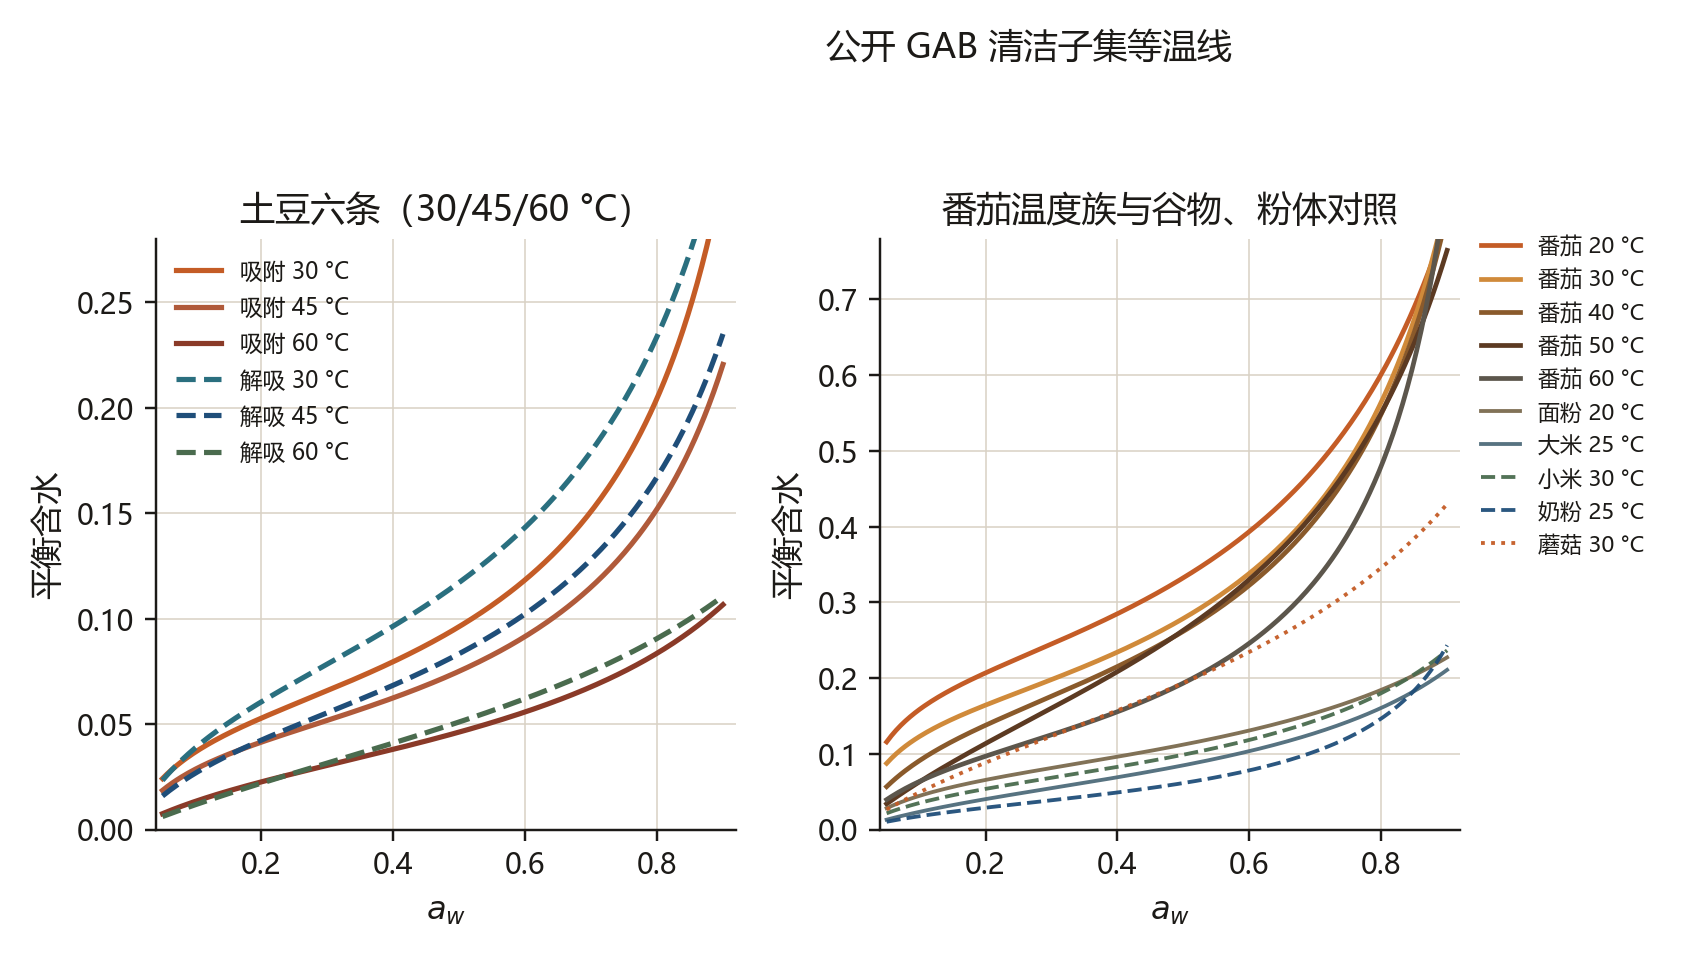
\includegraphics[width=0.9\textwidth]{paper/P_gab.png}
\caption{六条土豆清洁拟合在 \(a_w\in[0.05,0.90]\) 上的平衡含水。同一温度上脱附支高于吸附支。\(60^\circ\mathrm{C}\) 的两条曲线明显更低。测定温度不超过 \(60^\circ\mathrm{C}\)。}
\end{figure}

\begin{figure}[ht]
\centering
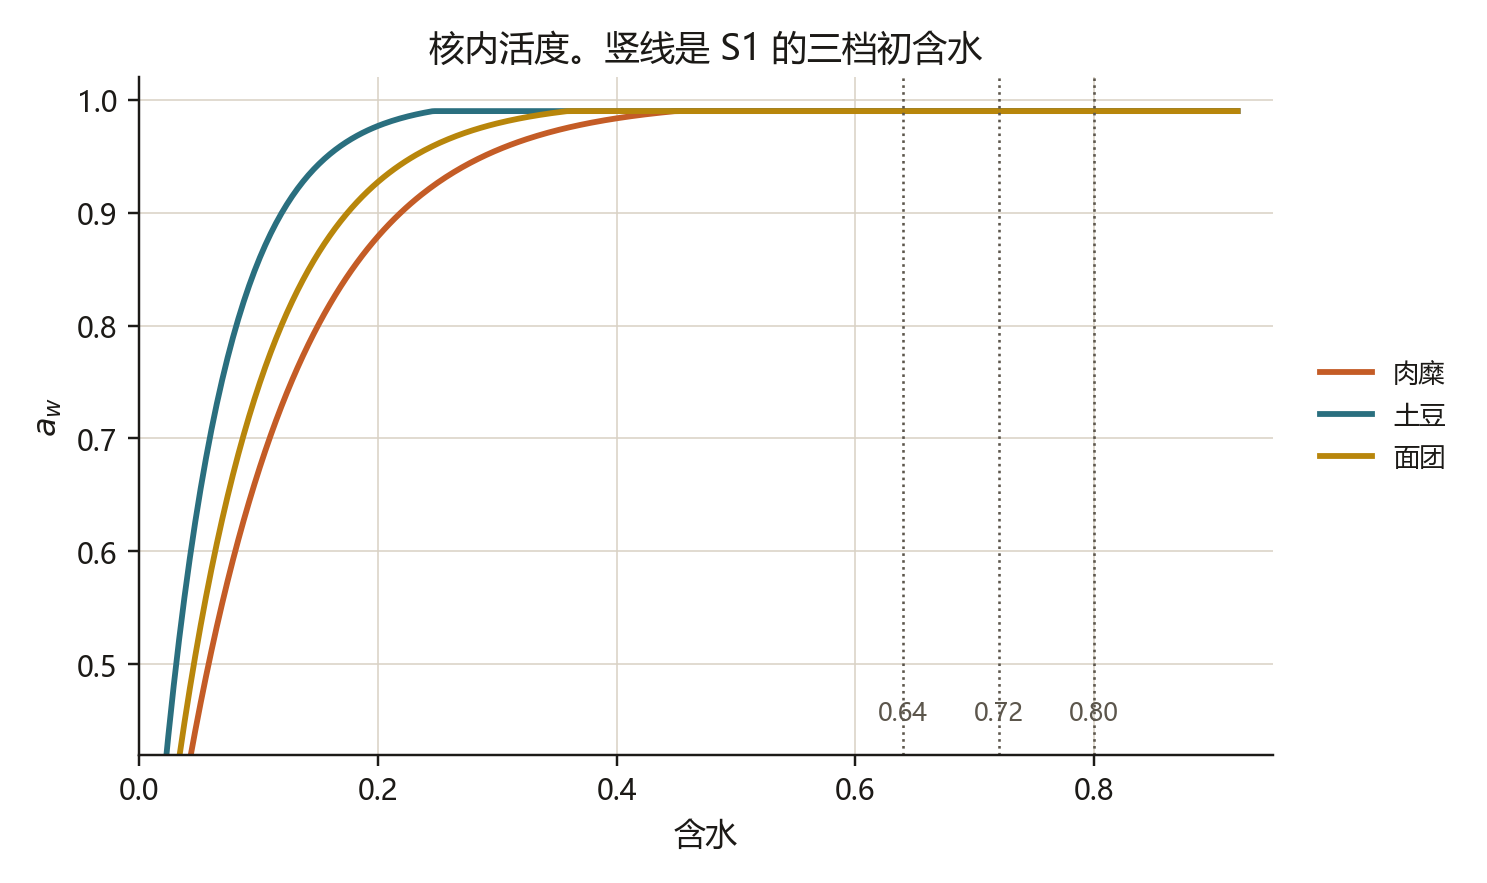
\includegraphics[width=0.88\textwidth]{paper/P_aw.png}
\caption{评分核的活度映射。竖线是 S1 的三档初含水。三条曲线在这三档上都贴近上界，所以食材因子在交叉表里几乎重合。}
\end{figure}

有效导热写成各向异性张量：
\begin{equation}
\label{eq:aniso}
\vect{k}_{\mathrm{eff}}=k_\perp(M,S)\,\vect{I}+(k_\parallel-k_\perp)\,\vect{e}\otimes\vect{e}.
\end{equation}
脂肪夹层作为并联热阻 \(R_{\mathrm{fat}}=L_{\mathrm{fat}}/(k_{\mathrm{fat}}A)\) 加到冷点路径上。冷点可以落在低导热层的背侧，而不必是几何中心。核里的非均质档 2 只把下标 5 的控制体导热乘 \(0.45\)，没有独立的脂肪几何，也没有纤维方向。

收缩：
\begin{equation}
\label{eq:shrink}
\dot L=-\beta_s L_0\,\dot\alpha_p,\qquad K=K_0\Big(\frac{L}{L_0}\Big)^{n_K}\varepsilon_g^{n_\varepsilon}.
\end{equation}
渗透率随孔隙与收缩一起变。核里的厚度在一条轨迹内是常数，收缩没有进入网格。

腔壁辐射用一个角系数：
\begin{equation}
q_{\mathrm{rad}}=F_{h,s}\epsilon_s\sigma(T_h^4-T_s^4)+F_{w,s}\epsilon_s\sigma(T_w^4-T_s^4).
\end{equation}
热像里的反射项与 \(F_{h,s}T_h^4\) 是同一几何量。核里没有这一项。

\paragraph{本节不能推出的结论}
闭合关系写在规格里，不能写成 S1 已经扫描了各向异性比或收缩指数。S1 的非均质只有两档：初始温度 \(\pm 4^\circ\mathrm{C}\)，以及一个控制体的导热系数。

\section{三个原型的方程差异}

\paragraph{要判定的量}
三个原型的差异来自哪一项开关，而不是来自三套互不相关的公式。

\begin{table}[ht]
\centering
\caption{原型开关}
\begin{tabularx}{\textwidth}{lXXX}
\toprule
项 & 肉糜 & 土豆 & 面团 \\
\midrule
主反应 & \(\alpha_p\) 与 \(\alpha_m\) & \(\alpha_g\)，需自由水 & \(\alpha_g\) 与后期 \(\alpha_b\) \\
等温线 & 开放区间，无公开肉类曲线 & 土豆清洁拟合，只到 \(60^\circ\mathrm{C}\) & 谷物清洁拟合的区间 \\
各向异性 & 文献区间，未在本次扫描 & 近似各向同性 & 气孔方向可有弱各向异性 \\
脂肪层 & 规格中可开启；本次只有一个低导热控制体 & 关闭 & 关闭 \\
收缩 & 规格开启；本次厚度固定 & 弱 & 体积变化作为已知几何，不反解 \\
\bottomrule
\end{tabularx}
\end{table}

核里三个原型共用同一套导热和进度公式。差别只在活度尺度：肉糜 \((0.10,0.70)\)，土豆 \((0.055,0.80)\)，面团 \((0.08,0.75)\)。交叉表里三个食材的中位误差几乎相同，与“原型只改了一个弱的活度尺度”一致。这不能用来声称蛋白与淀粉的反应差异已经被检验。

\paragraph{本节不能推出的结论}
面团膨胀不在状态里。把它反解进估计，会把发酵气体和热加工认知绑成一个问题。本次没有这样做，也不报告膨胀误差。

\section{无量纲结构与尺度分离}

\paragraph{要判定的量}
短探针的持续时间是否落在冷点 Fourier 数远小于 1 的窗口内。

取厚度 \(L\)、外部温差和初始液相分数。\(\mathrm{Fo}=\alpha t/L^2\) 衡量内部导热是否追上边界。\(\mathrm{Bi}=hL/k\) 衡量外部对流是否主导表面梯度。\(\mathrm{Ko}=\Delta h_{\mathrm{vap}}\varepsilon_{l0}\rho_l/((\rho c)_{\mathrm{eff}}\Delta T)\) 衡量潜热相对显热的大小。

用核的常数，40 s 窗口、30 mm 的 Fourier 数是 \(8.9\times 10^{-3}\)；风机 \(0.4\) 时 30 mm 的 Biot 数是 \(1.5\)。蒸制阶段界面冷凝使表面先跃迁，冷点仍由 Fourier 数控制。损伤预算因此主要写在表面褐变和表面含水上。厚度增大使内部时间常数增大，窗口更宽，但表面响应对内部热阻的灵敏度下降。信息增益存在上界；上界低于停机所需的熵减时，输出进度区间，不输出一个剩余时间点。本次没有计算这个上界的等高线。

\subsection{用已定常数算出的三张尺度图}

\begin{figure}[ht]
\centering
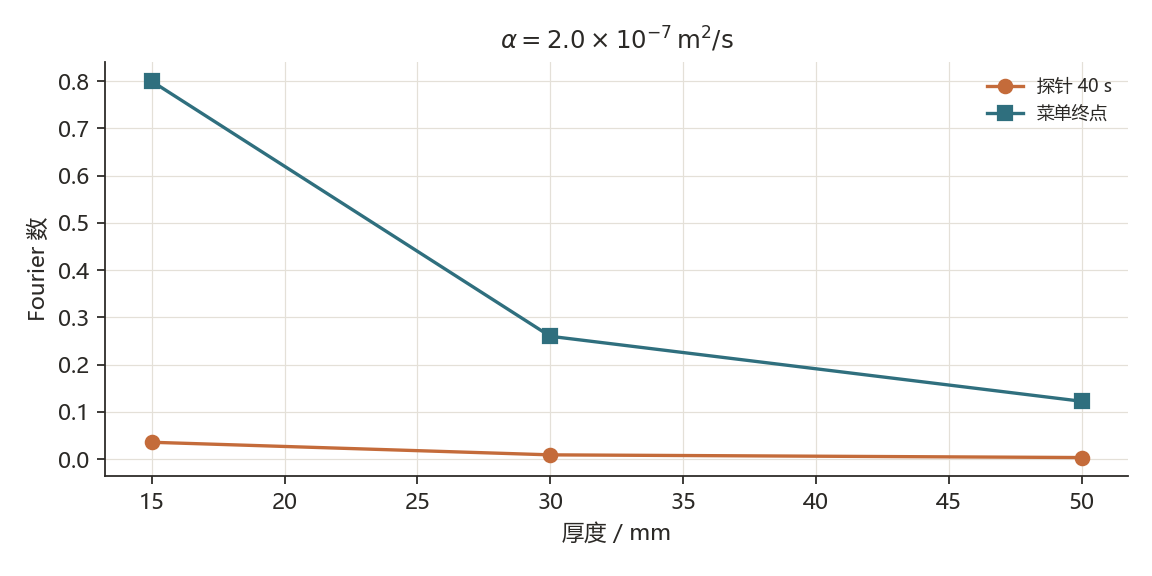
\includegraphics[width=0.88\textwidth]{paper/P_fo.png}
\caption{探针 40 s 与三档菜单终点的 Fourier 数。厚件在菜单终点仍远小于 1。\(\alpha\) 是核里的设定值。}
\end{figure}

\begin{figure}[ht]
\centering
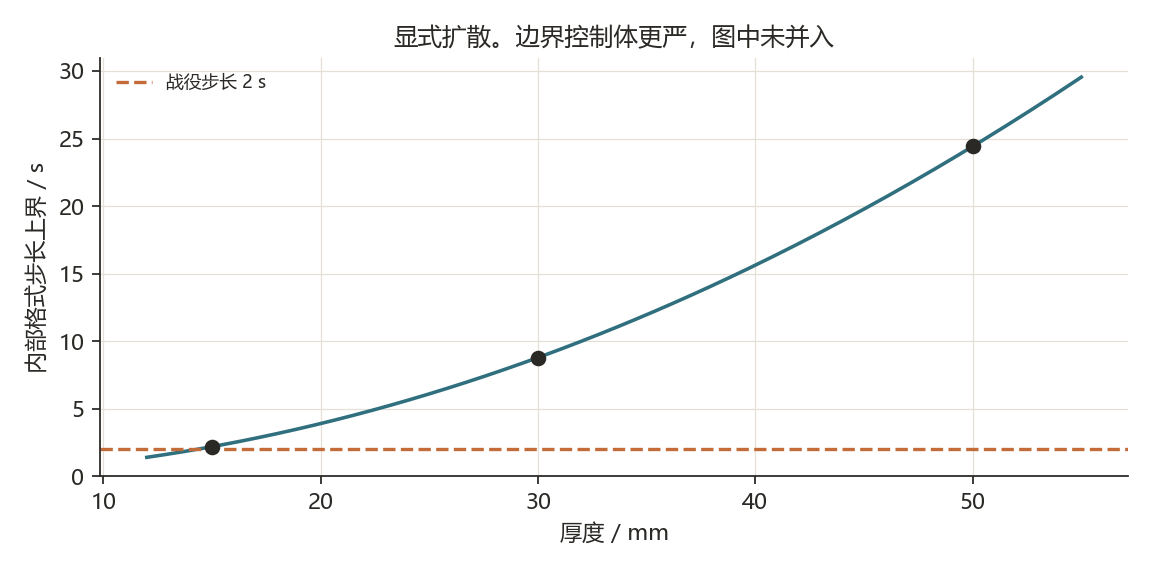
\includegraphics[width=0.88\textwidth]{paper/P_dt.png}
\caption{内部显式格式的步长上界。15 mm 处上界略高于战役使用的 2 s。边界对流项的上界更松，谱半径由内部差分决定。}
\end{figure}

\begin{figure}[ht]
\centering
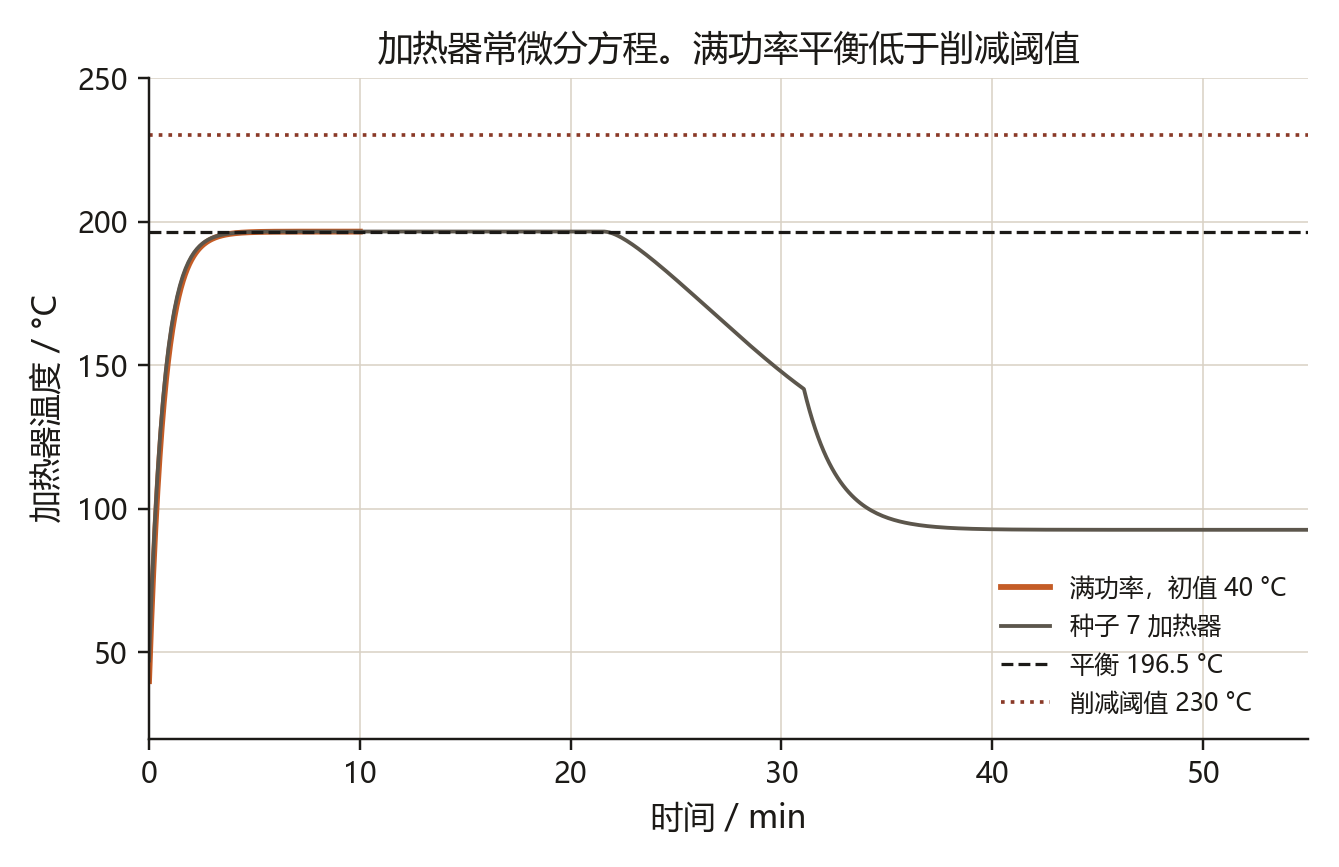
\includegraphics[width=0.88\textwidth]{paper/P_heater.png}
\caption{满功率加热器常微分方程从 \(40^\circ\mathrm{C}\) 出发，平衡在 \(196.5^\circ\mathrm{C}\)。削减阈值 \(230^\circ\mathrm{C}\) 在这条解上没有交点。}
\end{figure}

\subsection{常物性平板的本征根}

把核里的 \(\alpha\) 和 \(h\) 放进一块常物性、常换热、无潜热的平板，只为了给出线性对照。对照不是十六条格式的解。坐标从绝热面量到加热面，厚度仍是 \(L\)。无量纲温度 \(\theta\) 满足
\begin{equation}
\label{eq:slab}
\partial_{\mathrm{Fo}}\theta=\partial_{\xi\xi}\theta,
\qquad
\partial_\xi\theta\big|_{\xi=0}=0,
\qquad
\partial_\xi\theta\big|_{\xi=1}=-\mathrm{Bi}\,\theta(1).
\end{equation}
\(\xi=x/L\)，\(\mathrm{Fo}=\alpha t/L^2\)，\(\mathrm{Bi}=hL/k\)。分离变量 \(\theta=\cos(\zeta\xi)\,\mathrm{e}^{-\zeta^2\mathrm{Fo}}\) 放进加热面的边界条件，得到
\begin{equation}
\label{eq:slab-root}
\zeta\tan\zeta=\mathrm{Bi}.
\end{equation}
根落在 \((n\pi,\,n\pi+\pi/2)\)。均匀初温的系数由本征函数在 \([0,1]\) 上的权 \(\cos^2(\zeta\xi)\) 归一，第一项是
\begin{equation}
\label{eq:slab-A}
A_1=\frac{4\sin\zeta_1}{2\zeta_1+\sin 2\zeta_1}.
\end{equation}
第一项单独衰减的时间是 \(L^2/(\alpha\zeta_1^2)\)。下表的根用二分法求到 \(10^{-12}\) 量级，再四舍五入。

\begin{table}[ht]
\centering
\caption{常物性平板的前三个根。线性对照，不是核的轨迹。}
\begin{tabular}{lrrrr}
\toprule
条件 & \(\mathrm{Bi}\) & \(\zeta_1\) & \(\zeta_2\) & \(\zeta_3\) \\
\midrule
15 mm，风机 0.4 & 0.75 & 0.771 & 3.361 & 6.400 \\
30 mm，风机 0.4 & 1.50 & 0.988 & 3.542 & 6.510 \\
50 mm，风机 0.4 & 2.50 & 1.142 & 3.732 & 6.643 \\
30 mm，探针风机 1.3 & 3.68 & 1.245 & 3.899 & 6.781 \\
\bottomrule
\end{tabular}
\end{table}

对应的 \(A_1\) 是 1.097、1.154、1.197、1.224。第一项的时间：Bi \(=1.50\) 时，15 mm、30 mm、50 mm 分别是 1152 s、4608 s、12799 s。菜单终点的 Fourier 数是 0.80、0.26、0.12，都短于“第一项降到 \(1/\mathrm{e}\)”所需的 Fourier 数 1.02。六项截断下，中心剩余温差在探针窗口 \(\mathrm{Fo}=8.9\times 10^{-3}\)、Bi \(=1.50\) 时仍是 0.9997，表面剩余是 0.858。菜单终点上，15 mm（Bi \(=0.75\)，Fo \(=0.80\)）的中心剩余是 0.681，30 mm（Bi \(=1.50\)，Fo \(=0.26\)）是 0.887，50 mm（Bi \(=2.50\)，Fo \(=0.12\)）是 0.974。厚件在菜单时间上，常物性中心几乎还没动。这和交叉表里厚件开环停在进度下沿的方向相同。相同只说明尺度，因为核的腔温随加热指令从 \(90^\circ\mathrm{C}\) 变到 \(185^\circ\mathrm{C}\)，还有潜热项，初温也不必均匀。

\paragraph{本节不能推出的结论}
无量纲估计不能代替第 \ref{ch:sim} 章的策略比较。尺度使用的 \(\alpha\) 是设定值。更换 \(\alpha\) 之后的排序没有运行。本征根表不能读成种子 7 的剖面：那条轨迹的表面在 160 s 已经到 \(80^\circ\mathrm{C}\)，冷点仍在 \(8^\circ\mathrm{C}\)，驱动是随时间变化的通量，不是一次常 Bi 的阶跃。
